\chapter{Classification}\label{ml}

Previously, Chapters \ref{gle} and \ref{sce} demonstrate that both \gls{gle} and \gls{sce} contributed to characterising the cancer mutagenesis patterns. Chapter \ref{gle} shows that the smooth representation of GLE was better at discriminating cancers than the bin representation. Chapter \ref{sce} shows evidence that there is an informational advantage in exploiting the bases beyond 3-mers, namely flanking positions -2 and +2 with respect to the substitutions. 

Nonetheless, to manipulate the information from GLE and SCE, they have to be represented correctly. A sensible instinct is that a more suitable representation of a feature gives higher accuracy than a less suitable representation. This chapter acts as both an application and a validation for chapters \ref{gle} and \ref{sce}. In particular, section \ref{ml:gle} shows that smoothing GLE is a better representation than binning it. Section \ref{ml:sce} shows that currently strand symmetric 3-mer is the preferable representation of SCE. Additionally, section \ref{ml:both} demonstrates we can combine two factors with different units, like GLE and SCE, in a joint model in an attempt to further improve accuracy and to weigh the importance of each in the presence of the other.

While each of the next sections works on different data inputs, all sections follow the same procedure for training the classifier (Methods \ref{methods:ml_workflow}). Briefly, a small proportion of data is set aside as a test set, which is then used to evaluate model performance.

\section{Classifier based on GLE}\label{ml:gle}
This section seeks to identify the best approach to extract information from GLE for cancer prediction. Specifically, similar to section \ref{gle:bootstrap} of Chapter \ref{gle}, I trialled the bin \textit{v.s.} smooth representations together with the Euclidean \textit{v.s.} Wasserstein distances. Again, the conventional bin representation counts mutations in discrete segments of the genome while the smooth representation computes the density of genomic locations based on how dense mutations are distributed in the neighbourhood. The Euclidean distance between two vectors aggregates the differences between points at the same coordinates on the vectors while the Wasserstein distance allows comparing points at different coordinates. More detailed comparisons between the two representations and distance measures can be found in Methods \ref{methods:bootstrap}. For each representation and distance, I trained a KNN classifier with 1/10 of the donors being used as the test set. Comparing the observations in the test set to the predictions made by the classifier allowed calculating the accuracy measure $F1$. I iterated the training procedures 10 times to estimate the range of the $F1$ scores obtained from these approaches. $F1$ was chosen as the accuracy measure as it takes into consideration both sensitivity and specificity. Details about the training procedures can be found in Methods \ref{methods:ml_workflow}.

The results are summarised in Figure \ref{fig:f1_gle}. For the Euclidean distance, the smooth representation was much better than the bin approach in predicting cancers. This is also very clear when inspecting the confusion matrices (Figure \ref{fig:confusion_bin_euclidean} \textit{v.s.} \ref{fig:confusion_smooth_euclidean}), where many more observations lay on the diagonals for the smooth representation compared to the bin representation. This is consistent with the bootstrap results from section \ref{gle:bootstrap}, where the difference in GLE between cancers was more significant for the smooth representation than the bin representation. For the Wasserstein distance, the difference between the smoothing and bin approach was not obvious (Figure \ref{fig:f1_gle} and \ref{}). Besides, the $F1$ scores for both representations with the Wasserstein distance were about the same as that for the smooth representation with the Euclidean distance. This suggests that the properties of the Wasserstein distance allows it to alleviate the pitfalls introduced by the bin representation, which will be discussed in details in Section \ref{} of Chapter \ref{discussion}. 

\begin{figure}[htbp]
    \begin{subfigure}{.5\textwidth}
    \centering
    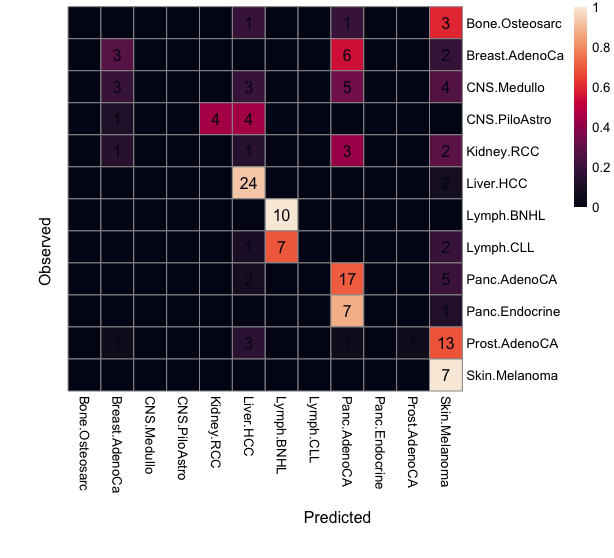
\includegraphics[width=\textwidth,height=0.9\textwidth]{graphics/confusion_matrix_bins_euclidean.png}
    \caption{Bin/Euclidean}
    \label{fig:confusion_bin_euclidean}
    \end{subfigure}
    ~
    \begin{subfigure}{.5\textwidth}
    \centering
    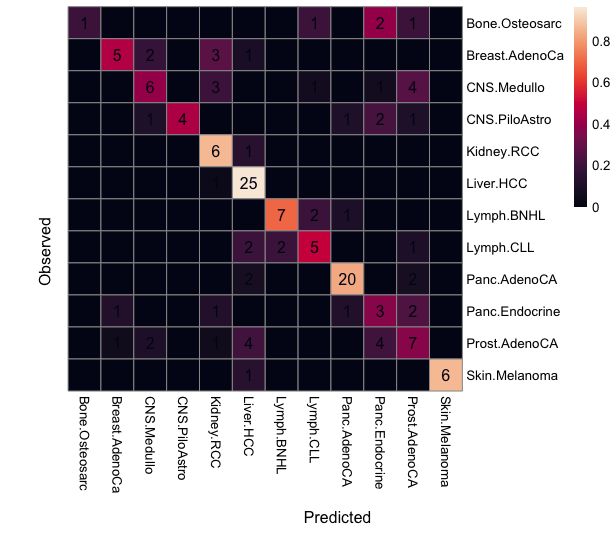
\includegraphics[width=\textwidth,height=0.9\textwidth]{graphics/confusion_matrix_smooth_euclidean.png}
    \caption{Smoothing/Euclidean}
    \label{fig:confusion_smooth_euclidean}
    \end{subfigure} \\
    \vspace{0.5cm}
    
    \begin{subfigure}{0.5\textwidth}
    \centering
    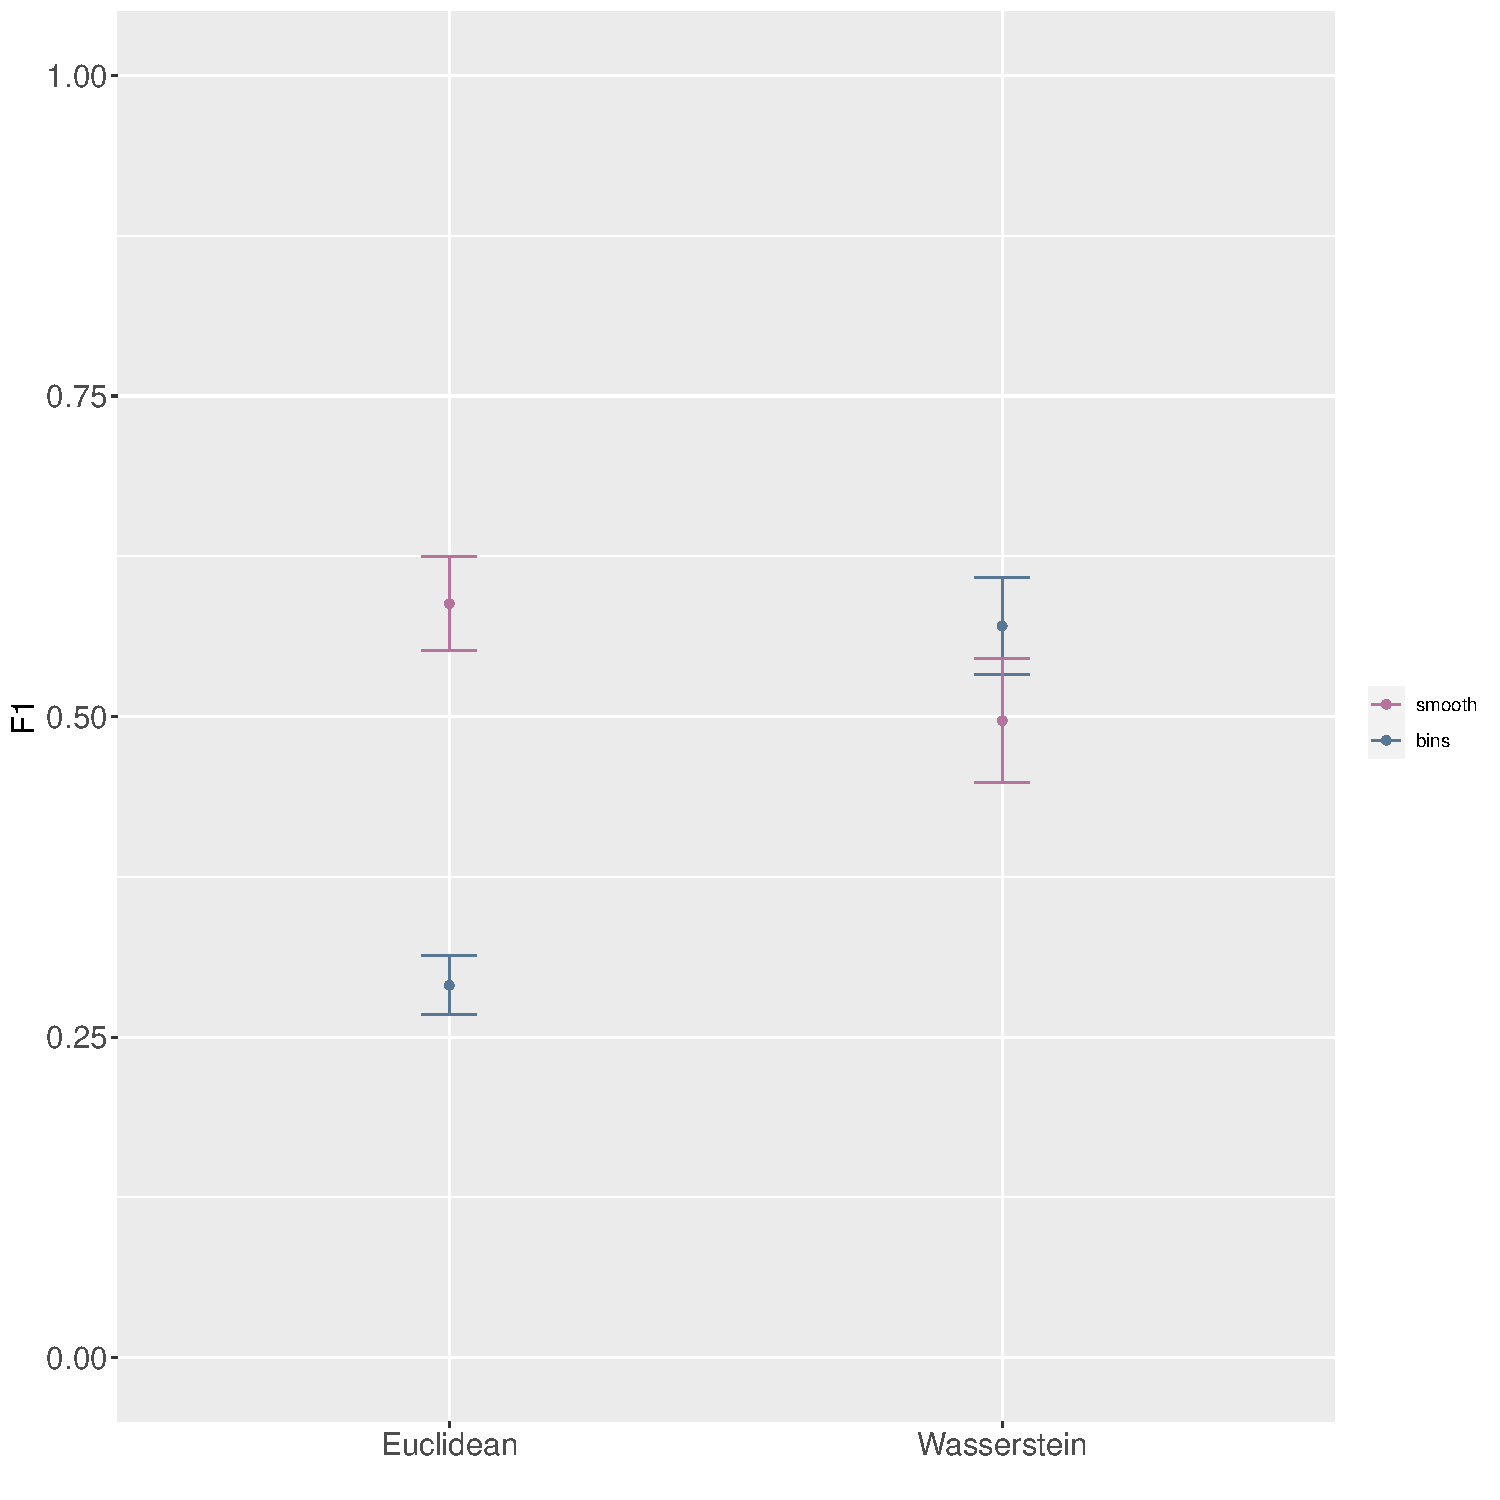
\includegraphics[scale=0.8]{graphics/f1_gle.pdf}
    \caption{F1 summary}
    \label{fig:f1_gle}
    \end{subfigure}
    
    
    \caption{\textbf{Smoothing was more accurate than binning for Euclidean distance, the difference between two representations was unclear for Wasserstein}. For each combination of representation/metric, I iterated the training procedures 10 times. Here, a representative confusion matrix, coloured by the percentage of predicted values over row total, is shown for (a) Bin/Euclidean, (b) Smooth/Euclidean. (c) shows the means of $F1$ for all representations/measures, the error bars are the standard errors for the iterated $F1$'s.}
    \label{fig:ml_gle}
\end{figure}

\section{Classifier based on SCE}\label{ml:sce}

\subsection{3-mer is the most accurate sequence context size}
To train a classifier based on SCE, I experimented with incorporating the flanking bases to the mutation composition, including the context sizes of 1-mer, 3-mer and 5-mer, where 1-mer is the base substitution without any context. In parallel, I trialled imposing asymmetry (no symmetry), semi-symmetry (reverse complementary strand symmetry) and full-symmetry (reverse complementary strand symmetry and flanking bases restricted to be A and C). Figure \ref{fig:f1_sce} shows the $F1$ for these approaches. In general, SCE was more accurate then GLE. However, the fully symmetric representation severely dropped in accuracy when flanking bases were involved, which suggests that it introduced noise to the data. Asymmetry and semi-symmetry performed roughly similarly, with 3-mer being the most accurate representation, reinforcing the evidence of strand symmetry previously seen in \ref{sce}. Assuming asymmetry and semi-symmetry is equivalent, $F1$ being lower for 5-mer than 3-mer but higher for semi-symmetry than asymmetry is very curious. It suggests the potential impact of splitting up mutation counts into too many elements in 5-mer (Table \ref{tab:sce_symmetric}).

\begin{figure}[h!]
    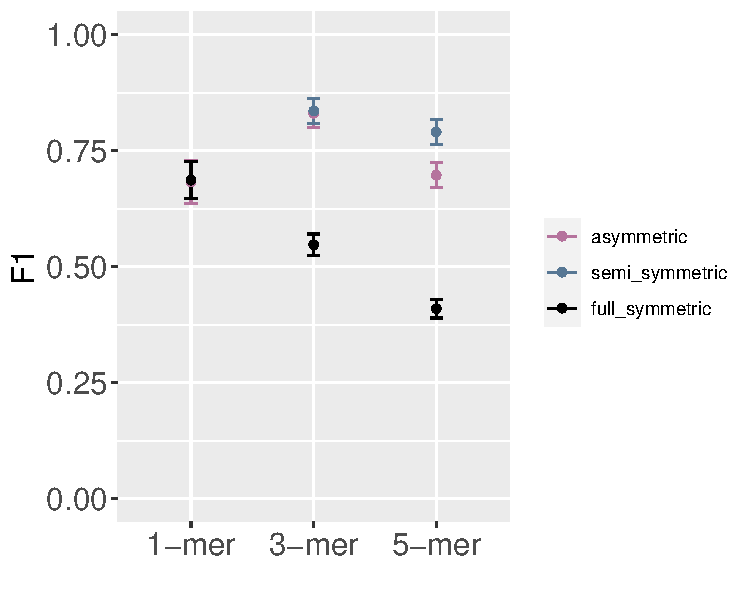
\includegraphics[scale=0.75]{graphics/f1_sce.pdf}
    \caption{\textbf{SCE classifiers using the 3-mer context  were the most accurate}. For each combination of representation/metric, I iterated the training procedures of the KNN classifier 10 times using Jensen-Shannon distance. The performance of the classifier was computed based on a previously held out test data set and reported as confusion matrices and $F1$'s. The y-axis is the means of $F1$ for 1-mer, 3-mer \& 5-mer and asymmetry, semi-symmetry \& full-symmetry; the error bars are the standard errors for the iterated $F1$’s. The corresponding confusion matrices are shown in Figure \ref{fig:apdx_ml_sce}.}
    \label{fig:f1_sce}
\end{figure}


\subsection{Dissecting 5-mer into submotifs can potentially improve accuracy}
Suspecting that the poor performance of 5-mer was due to the long vector that represented it, I tried splitting up 5-mers into smaller vectors (submotifs) then using the linear combination of them as input into the classifier (Table \ref{tab:submotif}). To demonstrate, for 2-submotifs, I split the long 5-mer vector into 4 shorter vectors that only involved 2 positions, including the base substitution. Figure \ref{fig:f1_sce_submotif} shows that the splitting did improve $F1$ compared to the original whole 5-mer vector, particularly the 3-submotif representation. This is very promising, but at this point it is uncertain whether it was the information from outer flanking positions or the 3-mer incorporated in the 3-motifs that drove this accuracy improvement.

\begin{figure}[h!]
    \centering
    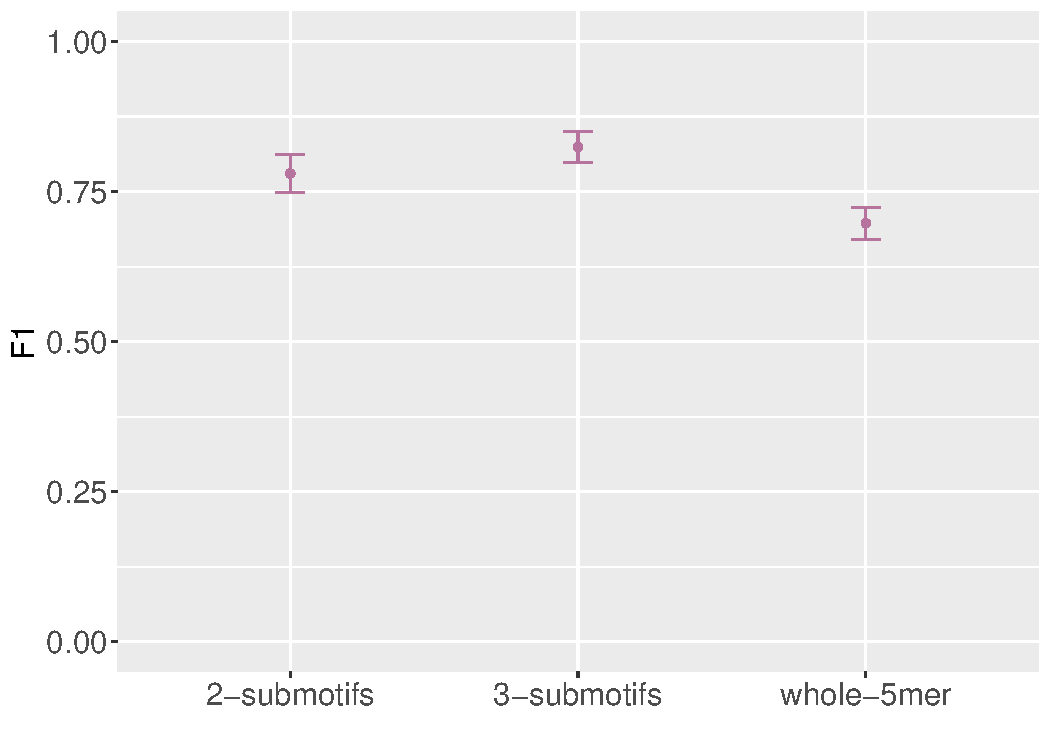
\includegraphics[scale=1]{graphics/f1_sce_submotif.pdf}
    \caption{\textbf{Dissecting 5-mer into multiple submotifs can potentially improve prediction accuracy compared to whole 5-mer}. For each combination of representation, I iterated the training procedures 10 times. The y-axis is the means of $F1$ for all representations/measures, the error bars are the standard errors for the iterated $F1$'s.}
    \label{fig:f1_sce_submotif}
\end{figure}


\section{Classifier based on the combination of GLE and SCE}\label{ml:both}
In this section, I attempted to combine GLE and SCE to see whether the combination could improve the accuracy over each factor by itself. I used (1) the conventional approach, which combined the bin representation for GLE and the semi-symmetric 3-mer representation for SCE as well as (2) my proposed approach, which combined the smooth representation for GLE and the asymmetric 3-mer representation for SCE. I trialled different weights on the two factors and reported $F1$ in Figure \ref{fig:f1_combined}. For both approaches, $F1$ improved for GLE but not SCE - accuracy was predominated by SCE. This is particularly true for the conventional approach. Even though model performance was not improved, this analysis shows that SCE is the stronger than SCE as a determinant of cancer.

\begin{figure}[h!]
    \centering
    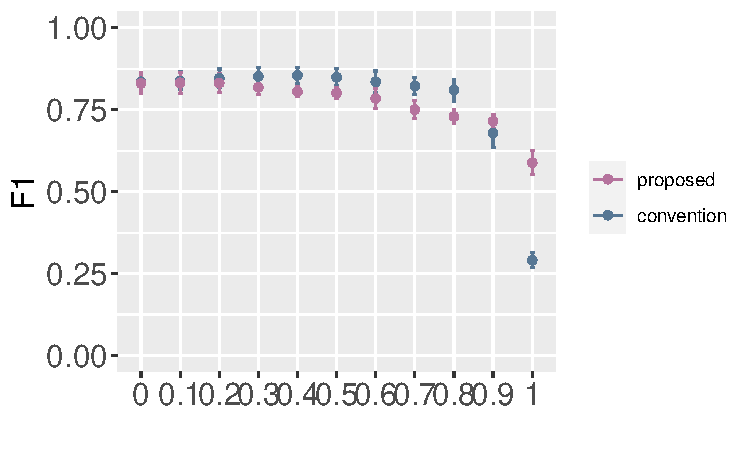
\includegraphics[scale=0.7]{graphics/f1_combined.pdf}
    \caption{\textbf{SCE was the stronger predictor of cancer prediction}. I combined GLE and SCE using two approaches: the conventional approach (bin for GLE and semi-symmetric 3-mer for SCE) and the proposed approach (smooth for GLE and asymmetric 3-mer for SCE). I used Euclidean distance for GLE and Jensen-Shannon distance for SCE. The x-axis is the weight given to GLE $g$, the weight given to SCE is accordingly $1-g$. For each weight combination, I iterated the training procedures 10 times. The y-axis is the means of $F1$ for all representations, the error bars are the standard errors for the iterated $F1$'s.}
    \label{fig:f1_combined}
\end{figure}


\section{Chapter summary}